\documentclass{ctexart}

\usepackage{amsmath}

\usepackage{amsthm}

\usepackage{amssymb}

\begin{titlepage}

\title{微分方程数值解 \\ 作业(一)}

\author{于慧倩 \\ 14300180118}

\date{2017年3月}

\end{titlepage}

\begin{document}

\maketitle

\newpage

\begin{enumerate}

%第一题

\item 计算
\(\displaystyle f(x)=\frac{1-\cos(x)}{x^2}\)
当\(x\)趋于0的时候的结果。

对\(x=(-4:0,1:4)\times10^{-8}\),画出\(f(x)\)的图像:

\centerline{\includegraphics[width=5.5in]{Ch1_Ex1.eps}}

\(\displaystyle f(x)=\frac{1-\cos(x)}{x^2}\)在当\(x\)趋于0的时候函数值在0.5附近震荡,且愈靠近0处震荡愈显著,在\(x=0\)邻域内分子为0,\(f(x)=0\),且\(x=0\)点无意义。由于\(x\)趋于0的时候,1与\(\cos(x)\)符号相同、数值相近,二者相减使分子的有效数字减少信息缺失,导致整体相对误差的放大。

%第二题

\item 考虑倒向迭代过程,则舍入误差可以被很好的控制:

\begin{proof}

由递推公式得到\(u_n\)可以表示为
\[u_n=c_1 2^n + c_2 1^n. \]

\(c_1 , c_2\)由初始值\(u_N , u_{N-1}\)给定:
\begin{itemize}

\item  如果\(u_N=u_{N-1}\),则\(u_1=u_N\).

\item 如果\(u_N \neq u_{N-1}\),则

\[ u_n=(u_N-u_{N-1})2^{n+1-N}+(2u_{N-1}-u_N). \]

\end{itemize}

由上一节实验知
\begin{eqnarray*}
a_0  &\triangleq&  3\times \mbox{double}(0.1) - 2\times \mbox{double}(0.1) - \mbox{double}(0.1) \nonumber \\
      &=&  2.7756e-17(=2^{-55}). \nonumber
\end{eqnarray*}

这样在\(u_{N-2}\)就会有舍入误差引入,不妨把迭代格式看成从\(n=N-3\)开始,且初值为\(u_{N-1},u_{N-2}\),并假设后续的计算是在一个理想的没有舍入误差的计算机中运行,则第\(N-2-n\) 步的值\(u_n\)为
\[ \tilde{u}=\mbox{double}(0.1)+a_0 \times 2^{n+1-N}-a_0\]

对于迭代次数很大的对应的很小的\(n\)误差维持在1左右,\(n\)较大时(且\(n \leq N-2\)时)最大值小于
\(  \frac{3}{2}\):
\[ 1.5 \geq  \frac{|u_{n}-0.1|}{|u_{n+1}-0.1|} \approx 1\]

可以从下图观察到。

\centerline{\includegraphics[width=5in]{Ch1_Ex2.eps}}

 \end{proof}
 
 %第二种证明
 
 \begin{proof}
 
 上述分析不考虑在计算\(\frac{3}{2}u_{N-1}-\frac{1}{2}u_N\)时引入的舍入误差,只考虑在初始时刻的扰动。实际上每一步计算时,递推公式都会有舍入误差存在。不妨假设实际的计算格式可以写为原来计算格式的扰动:
 \[\tilde{u}_n=\frac{3}{2}\tilde{u}_{n+1}-\frac{1}{2}\tilde{u}_{n+2}+\epsilon_n\]
 
 且初始值为
 \[ \tilde{u}_N=u_N+\epsilon_N, \tilde{u}_{N-1}=u_{N-1}+\epsilon_{N-1}\]
 
 定义向量
 
 \[\boldsymbol{ \omega}_n={u_{n+1}\choose u_n}, \tilde{\boldsymbol{ \omega}}_n={\tilde{u}_{n+1}\choose \tilde{u}_n},
 \boldsymbol{\varepsilon}_n={\epsilon_{n+1}\choose 0} \]
  
  则递推公式可以写为单步递推公式:
 \[ \boldsymbol{ \omega}_n=\boldsymbol{A}\boldsymbol{ \omega}_{n+1}\]
 
 和
 \[\tilde{\boldsymbol{ \omega}}_n=\boldsymbol{A}\tilde{\boldsymbol{ \omega}}_{n+1}+\boldsymbol{\varepsilon}_n\]
 
 这里矩阵\(\boldsymbol{A}\)为
 \[\boldsymbol{A}=\left(                 %左括号
  \begin{array}{cc}   %该矩阵一共3列,每一列都居中放置
    0 & 1 \\  %第一行元素
    -\frac{1}{2} & \frac{3}{2} \\  %第二行元素
  \end{array}
\right) \]

定义误差\(\boldsymbol{e}_n=\tilde{\boldsymbol{ \omega}}_n - \boldsymbol{ \omega}_n\),则对\(n \geq N-2\)有:
\begin{eqnarray}
\boldsymbol{e}_n &=& \boldsymbol{A}(\tilde{\boldsymbol{ \omega}}_{n+1}-\boldsymbol{ \omega}_{n+1})+\boldsymbol{\varepsilon}_n \nonumber \\
      &=& \boldsymbol{A}\boldsymbol{e}_{n+1}+\boldsymbol{\varepsilon}_n \nonumber
\end{eqnarray}

另外定义\(\boldsymbol{e}_{N-1}={\epsilon_N \choose \epsilon_{N-1}}\)。容易得到矩阵\(\boldsymbol{A}\)的特征值分解:
\[ \boldsymbol{P}^{-1}\boldsymbol{A}\boldsymbol{P}=\boldsymbol{\Lambda},
 \boldsymbol{P}=\left(                 %左括号
  \begin{array}{cc}   %该矩阵一共3列,每一列都居中放置
    -0.8944& -0.7071\\  %第一行元素
    -0.4472 &-0.7071\\  %第二行元素
  \end{array}
  \right) ,
\boldsymbol{\Lambda}=\left(                 %左括号
  \begin{array}{cc}   %该矩阵一共3列,每一列都居中放置
    0.5 & \\  %第一行元素
    &1\\  %第二行元素
  \end{array}
\right) 
\]

因此,误差的递推公式可以写成:
\[\boldsymbol{P}^{-1}\boldsymbol{e}_n=\boldsymbol{\Lambda} \boldsymbol{P}^{-1}\boldsymbol{e}_{n+1}+\boldsymbol{P}^{-1}\boldsymbol{\varepsilon}_n.\]
进而得到:
\[ \boldsymbol{P}^{-1}\boldsymbol{e}_n=\boldsymbol{P}^{-1}\boldsymbol{\varepsilon}_n+\boldsymbol{\Lambda} \boldsymbol{P}^{-1}\boldsymbol{\varepsilon}_{n+1} + \dots+\boldsymbol{\Lambda}^{N-n-2}\boldsymbol{P}^{-1}\boldsymbol{\varepsilon}_{N-2}+\boldsymbol{\Lambda}^{N-n-1}\boldsymbol{P}^{-1}e_{N-1}.\]

假设在每一步递推中\(\epsilon_i\)足够小,或假设:
\[ \|\boldsymbol{P}^{-1} \boldsymbol{\varepsilon}_i\| \leq \delta,\|\boldsymbol{P}^{-1}\boldsymbol{e}_{N-1}\| \leq \delta \]

则由上述递推公式容易得到:
\[ \|\boldsymbol{P}^{-1}\boldsymbol{e}_n\| \leq  (\underbrace{1^0+1^1+1^2+\dots +1^{N-n-1}}_{(N-n) \mbox{个}})\delta = (N-n)\delta\]

对任意向量\(\boldsymbol{v}=(v_1,\dots,v_d)^T, |v_i| \leq \| \boldsymbol{v}\| \),这样得到:
\[
|u_n-\tilde{u}_n| \leq \|\boldsymbol{P}\| \|\boldsymbol{P}^{-1}\boldsymbol{e}_n\| < 1.3960 \times (N-n)\delta.\]

\[ \frac{|u_n-\tilde{u}_n|}{|u_{n+1}-\tilde{u}_{n+1}|} = \frac{N-n}{N-n-1}\]

因此在迭代初期(\(n\)较大时),每迭代一次,增加误差大于1倍但相对较小,在迭代后期(\(n\)较小时),迭代过程中误差几乎不变,所以舍入误差在整个计算过程中可以被很好的控制。

\end{proof}

%第三题

\item 知
\[\| x_{n+2} - x_{n+1}\| \leq \alpha \|x_{n+1} - x_n\|  \ \ 0 \leq \alpha \leq1\]

进一步推导出
\[ \| x^* - x_n\| \leq \frac{\alpha^n}{1-\alpha} \|x_1 - x_0\| \]

\begin{proof}

\begin{eqnarray}
 \| x^* - x_n\|  &\leq& \alpha^1 \|x^* - x_{n-1}\|  \nonumber \\
                     &\leq& \alpha^2 \|x^* - x_{n-2}\|    \nonumber \\
                     &\dots& \nonumber \\
                     &\leq& \alpha^{n-1} \|x^* - x_1\|    \nonumber \\
                     &\leq& \alpha^{n} \|x^* - x_0\|     
\end{eqnarray}

 对于所有N:
 \begin{eqnarray}
 \|x_n - x_{n-1}\| &\leq&  \alpha^1 \|x_{n-1} - x_{n-2}\|  \nonumber \\
                          &\leq&  \alpha^2 \|x_{n-2} - x_{n-3}\|  \nonumber \\
                          &\dots& \nonumber \\
                          &\leq&  \alpha^{n-1} \|x_1 - x_0\|  
 \end{eqnarray}
  
 对于所有M:
 \begin{eqnarray}
 \|x_M-x_0\| &\leq& \|x_M - x_1\| + \| x_1 - x_0\| \nonumber \\
                     &\leq& \|x_M - x_2\| +\|x_2 - x_1\| + \| x_1 - x_0\| \nonumber \\
                     &\dots& \nonumber \\
                      &\leq& \|x_M - x_{M-1}\| + \| x_{M-1} - x_{M-2} \| + \dots +\|x_1 -x_0\|     \nonumber \\
                      &\leq& \|x_1 - x_0\|(1+\alpha+\alpha^2+\dots +\alpha^{M-1}) \nonumber \\
                      &=& \displaystyle \frac{1-\alpha^{M-1}}{1-\alpha}\|x_1 - x_0\| 
\end{eqnarray}

令\(x\rightarrow \infty\)得
\begin{equation}
 \|x_n - x_0\| \leq  \frac{1}{1-\alpha} \|x_1 - x_0\| 
\end{equation}

由(1)与(4)知:
 \begin{eqnarray*}
\|x^*-x_n\| &\leq&  \frac{\alpha^n}{1-\alpha}\|x_1 - x_0\| \\
                  &\leq& \ \frac{1}{1-\alpha}\|x_1 - x_0\| 
\end{eqnarray*}

\end{proof}
\end{enumerate}
\end{document}